% NAACL short paper draft. Compile: tectonic main.tex  (or pdflatex + bibtex)
% Numbers: looping_mechanism/results/paper_numbers.md (python looping_mechanism/paper_numbers.py)
\documentclass[11pt]{article}
\usepackage[review]{acl}
\usepackage{times}
\usepackage{latexsym}
\usepackage[T1]{fontenc}
\usepackage[utf8]{inputenc}
\usepackage{microtype}
\usepackage{inconsolata}
\usepackage{graphicx}
\usepackage{booktabs}
\usepackage{multirow}
\usepackage{xcolor}

\newcommand{\todo}[1]{\textcolor{red}{[TODO: #1]}}
\newcommand{\think}{\texttt{</think>}}

\title{Stopping Is Not Resolving: Why Reasoning Models Loop\\
When No Answer Fits}

\author{Anonymous submission}

\begin{document}
\maketitle

\begin{abstract}
Reasoning models sometimes never stop thinking, and common fixes simply force them to. We ask why
the loops arise and whether stopping them helps. Removing the valid answer from multiple-choice
questions makes DeepSeek-R1-Distill-Qwen-7B loop on 73--75\% of MATH, GSM8K and AQuA questions it
otherwise solves (vs.\ 2--9\%), and natural AQuA loops concentrate on questions whose open-ended
answer matches no option (30\% vs.\ 1\% of runs). In R1 and in Qwen3-4B-Thinking, the decision to
emit \think{} is made in late layers in the same way on four benchmarks, but this gate is generic:
it is as closed at healthy self-doubt as in loops. Opening it, by forcing \think{} or with an
internal switch learned on controlled loops and tested on held-out natural ones, ends loops without
resolving them: in a live test, stopping changes accuracy by $-5$ to $+30$ points and the switch
never beats forcing the token. Resolving the conflict works better: allowing ``None'' as an answer
removes half or more of the conflict loops with almost no cost on answerable questions.
\end{abstract}

\section{Introduction}
Large reasoning models (LRMs) think before they answer, and occasionally they do not stop: the trace
runs to the token budget, re-checking the same step, and no answer is produced
\citep{duan2026circular}. Practical remedies end the thinking from outside, by forcing the
end-of-thinking delimiter \citep[budget forcing;][]{muennighoff2025s1} or by steering the model out of
the loop \citep{yu2026sophia,zhang2026astray}, and are judged on whether the loop is broken. We ask
what triggers the loop and whether breaking it resolves whatever caused it.

Our contributions: (1) a controlled trigger: with no valid option, R1 loops on three quarters of
multiple-choice questions (MCQs) it can solve, on constructed and real questions, and the same
answer--option conflict predicts which natural questions loop (\S\ref{sec:when}); (2) a mechanism:
the \think{} decision is written by late layers, identically across four benchmarks, but the gate
is generic rather than suppressed in loops; it is concentrated in a few MLPs in R1 and spread over
late MLPs and attention in Qwen3 (\S\ref{sec:where}); (3) stopping is not resolving: in replay and in
a live test on held-out loops, every way of stopping ends the thinking but leaves the doubt, and the
internal switch never beats budget forcing (\S\ref{sec:fix}); (4) resolving is: allowing ``None''
removes most conflict loops (\S\ref{sec:resolve}).

\section{Setup}
\label{sec:setup}
\paragraph{Models and decoding.} DeepSeek-R1-Distill-Qwen-7B \citep[R1;][]{deepseek2025r1} and
Qwen3-4B-Thinking-2507 \citep{yang2025qwen3}, served with vLLM \citep{kwon2023vllm}, sampled with the
recommended $T{=}0.6$, top-$p$ 0.95, 4 seeds and a 12k-token budget; for R1 we also report greedy
decoding. A \textbf{loop} is a run that exhausts the budget without emitting \think{}.

\paragraph{Conditions.} Two-option MCQs built from 150 MATH \citep{hendrycks2021math} and 200 GSM8K
\citep{cobbe2021gsm8k} problems: \textsc{aligned} (correct number vs.\ an unrelated sentence) and
\textsc{catch} (a wrong number vs.\ a sentence: no valid option). To avoid an artificial distractor we
also pose 227 AQuA \citep{ling2017aqua} and 200 LogiQA \citep{liu2020logiqa} questions with the
correct option deleted, next to their original forms. Natural benchmarks are the datasets of
\citet{yu2026sophia} in native form: GSM8K, MATH-500, AQuA (5 options), LogiQA (4 options).

\paragraph{Learning and held-out testing.} For each benchmark and temperature, questions that loop
naturally in any seed are \emph{held out}. On the remaining questions we pair a \textsc{catch} run that
loops with the \textsc{aligned} run that finishes correctly (same question and seed) and compare the token
before \think{} in the finished run with the loop's \emph{commit point}, where, having just stated an
answer, it writes ``Wait'' (detected from the text without the answer key; hand-checked, Appendix).
Stop components and their values (the mean output at real stops) are learned from these pairs only.
We test on the held-out questions in two ways. \emph{Replay}: each natural loop is fed up to its commit
point and the intervention applied there. \emph{Live}: the held-out questions are generated afresh
with new seeds; a rule that reads only the text so far fires on any run with no \think{} after 6k
thinking tokens, at the next ``states a result, then doubts it'' point (fixed in advance, not tuned),
and every run it fires on, loop or not, is continued under each intervention. Answers (up to 1.2k
tokens after \think{}) are scored against the key.

\section{When do reasoning models loop?}
\label{sec:when}

\begin{table}[t]
\centering
\small
\setlength{\tabcolsep}{3.5pt}
\resizebox{\columnwidth}{!}{%
\begin{tabular}{llccc}
\toprule
 & valid? & R1 & R1 greedy & Qwen3 \\
\midrule
MATH-150 \textsc{aligned} & yes & 5.3 & 10.0 & 9.3 \\
MATH-150 \textsc{catch} & \textbf{no} & \textbf{74.7} & \textbf{98.0} & \textbf{29.5} \\
GSM8K-200 \textsc{aligned} & yes & 2.1 & 8.0 & 0.0 \\
GSM8K-200 \textsc{catch} & \textbf{no} & \textbf{73.4} & \textbf{100} & 0.2 \\
AQuA-227 original & yes & 8.5 & 25.1 & 2.9 \\
AQuA-227 correct removed & \textbf{no} & \textbf{74.4} & \textbf{93.8} & \textbf{9.0} \\
LogiQA-200 original & yes & 7.5 & 36.5 & 2.6 \\
LogiQA-200 correct removed & \textbf{no} & \textbf{15.0} & \textbf{42.0} & \textbf{10.1} \\
\midrule
GSM8K / MATH-500 (open) & yes & 0.4 / 5.2 & 4.2 / 10.0 & 0.1 / 15.3 \\
AQuA / LogiQA & yes & 7.9 / 9.5 & 25.6 / 39.4 & 2.9 / 3.2 \\
\bottomrule
\end{tabular}}
\caption{Loop rate (\%): the run never emits \think{} within 12k tokens. Sampled ($T{=}0.6$) rates are
means over 4 seeds. Top: the same questions with and without a valid option; bottom: natural
benchmarks.}
\label{tab:loops}
\end{table}

Removing the valid answer makes R1 loop on 73--75\% of MATH, GSM8K and AQuA runs, against 2--9\% on
the same questions with a valid option (Table~\ref{tab:loops}); greedy decoding raises both, to
94--100\% without a valid option. The traces are explicit: the model derives the answer, notes it is
not an option, re-derives it, and repeats. Runs that do finish pick a wrong option (82\% for MATH
\textsc{catch}, 100\% for AQuA) and never decline, as instruction-tuned models do
\citep{goral2025wait}. LogiQA, whose options are arguments rather than values, only doubles (7.5\% to
15\%). Qwen3 shows the same effect at a smaller scale (MATH 9\% to 30\%, AQuA 3\% to 9\%, LogiQA 3\% to
10\%) and handles GSM8K \textsc{catch} without looping.

\paragraph{Natural loops follow the same conflict.} We ask each model the AQuA questions with no options
and group them by its own answer. If that answer matches the correct option, the 5-option question
loops in 1\% of runs (R1; Qwen3 0\%); if it matches no option, through the model's own error or a noisy
key, it loops in 30\% (Qwen3 10\%). Natural MCQ loops are the controlled conflict, arising by itself.

\section{Where is the stop decided?}
\label{sec:where}

\begin{figure*}[t]
\centering
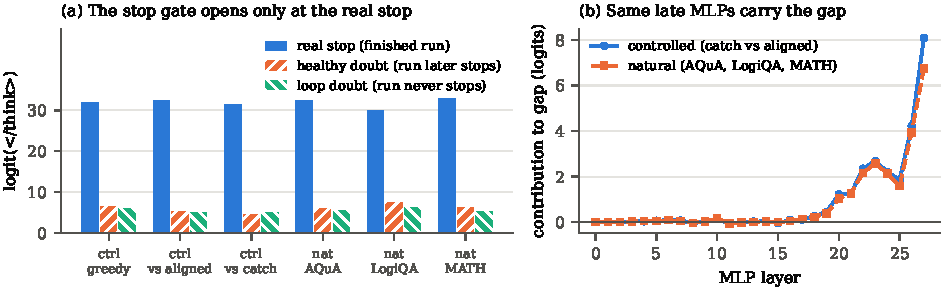
\includegraphics[width=\textwidth]{figures/stop_gate.pdf}
\caption{R1. (a) Logit of \think{} at the real stop of finished runs, at healthy doubts in finished runs
(an answer is stated, then ``Wait'', but the run later stops) and at the commit point of looping
runs. (b) Direct contribution of each MLP to the gap between the real stop and the loop's commit
point, for controlled and natural pairs.}
\label{fig:gate}
\end{figure*}

At a real stop \think{} has logit $\approx$+32 and is the top-1 token; at the loop's commit point it is
$\approx$+5 (gap $>0$ in 100\% of pairs). Direct logit attribution \citep{nostalgebraist2020lens,
nanda2022transformerlens} assigns about 90\% of R1's gap to MLPs. Learned separately on each
benchmark's own pairs (24--175 pairs per benchmark and temperature), the six MLPs carrying it are the
same in all eight settings (layers 22--27), the gap is +24 to +29, and replacing their output at the
commit point with the learned values recovers 78--98\% of it (control MLP: $\leq$1\%).

\paragraph{The gate is generic.} If loops suppressed the gate, the stop signal should be lower at a
loop's commit point than at a healthy doubt. It is not (Figure~\ref{fig:gate}a): at the same position,
loop doubts are +0.35 logits \emph{higher} (95\% CI 0.08--0.62), against $\approx$+26 for a real stop,
and across all natural loops the highest $P(\think)$ at any line break is $\approx$0.001 (median).
The late layers are the model's general ``stop now'' gate; a loop is a run that never reaches the state
that opens it.

\paragraph{Qwen3 spreads the gate.} Qwen3 shows the same gap (+27 to +28 on every benchmark), but only
59\% of it is written by MLPs and 41\% by attention in the last four layers; its six strongest MLPs
carry 47\%. Patching them recovers half the gap but never makes \think{} the top token. Patching all
MLPs from layer 18 recovers 83\% and makes it the top token in 93\% of pairs, and replacing the residual
stream at layer 21 or later recovers all of it: the decision is formed by layer 21 and written by many
late components.

\section{Does stopping fix loops?}
\label{sec:fix}

\begin{table}[t]
\centering
\small
\setlength{\tabcolsep}{3pt}
\resizebox{\columnwidth}{!}{%
\begin{tabular}{l|ccc|ccc|ccc}
\toprule
 & \multicolumn{3}{c|}{R1} & \multicolumn{3}{c|}{R1 greedy} & \multicolumn{3}{c}{Qwen3} \\
 & none & force & switch & none & force & switch & none & force & switch \\
\midrule
AQuA & 31 & 39 & 41 & 28 & 58 & 52 & 38 & 46 & 38 \\
LogiQA & 31 & 37 & 34 & 22 & 37 & 33 & 42 & 41 & 41 \\
MATH-500 & 45 & 40 & 40 & 42 & 44 & 46 & 34 & 60 & 34 \\
GSM8K & -- & -- & -- & 38 & 57 & 57 & -- & -- & -- \\
\bottomrule
\end{tabular}}
\caption{Live test: accuracy (\%) over fresh runs of the held-out questions (those that loop
naturally) when the stop rule may fire. none = no intervention; force = \think{}; switch = the
benchmark's own learned stop MLPs, set once. 95\% CIs are $\pm$8--13 points. Sampled GSM8K has too
few held-out questions (R1: 5, Qwen3: 1).}
\label{tab:fix}
\end{table}

\paragraph{Replay.} At the commit point of held-out natural loops, forcing \think{} ends every loop and
the learned switch 79--91\% of R1's, but answers are right for only 14--36\% (R1, $T{=}0.6$; switch
15--25\%), against 0\% if the loop is left alone. The doubt survives the stop: the answer often opens
with ``But wait'' and keeps re-checking until the answer budget runs out (45--86\% of answers). In
Qwen3 the switch stops 0\% of loops (forcing: 17--38\% correct), as its gate predicts. A broad patch of
all late MLPs does stop all 20 Qwen3 loops we tested, with 10\% correct, the same as forcing \think{}.

\paragraph{Live.} As a real stop rule (Table~\ref{tab:fix}), stopping helps on the MCQ benchmarks
(R1: +3 to +10 points) and hurts on MATH-500 at $T{=}0.6$ ($-5$): there the rule cuts short runs that
would have finished correctly (7) more often than it rescues loops (2). Gains are larger where loops
are runs that would have solved the problem: greedy loops, which are mostly repetition (AQuA 28\% to
58\%), and Qwen3's MATH loops, which mostly run out of budget (34\% to 60\%). Across all ten settings,
the internal switch is never better than forcing \think{} by more than 2 points, and on Qwen3 it never
fires. Opening the gate from inside adds nothing to opening it from outside.

\section{Resolving the conflict}
\label{sec:resolve}

\begin{table}[t]
\centering
\small
\setlength{\tabcolsep}{4pt}
\resizebox{\columnwidth}{!}{%
\begin{tabular}{l|cc|cc}
\toprule
 & \multicolumn{2}{c|}{R1} & \multicolumn{2}{c}{Qwen3} \\
no valid option & loops & ``None'' & loops & ``None'' \\
\midrule
MATH \textsc{catch} & 76 $\to$ \textbf{35} & 44 & 32 $\to$ \textbf{18} & 82 \\
GSM8K \textsc{catch} & 72 $\to$ \textbf{19} & 66 & 0 $\to$ 0 & 96 \\
AQuA, correct removed & 74 $\to$ \textbf{35} & 30 & 9 $\to$ \textbf{4} & 75 \\
LogiQA, correct removed & 16 $\to$ \textbf{8} & 20 & 10 $\to$ 8 & 18 \\
\bottomrule
\end{tabular}}
\caption{Allowing ``None'': loop rate (\%) without $\to$ with the added sentence, and the share of runs
answering ``None'' (2 seeds each).}
\label{tab:none}
\end{table}

If the conflict drives the loop, a legitimate way out should remove it where stopping did not. We add
one sentence to the prompt: ``If none of the options is correct, put None within \textbackslash
boxed\{\}.'' Loops fall by 50--74\% for R1 and by 44--56\% where Qwen3 loops (MATH, AQuA), and the model now often declines
(Table~\ref{tab:none}). The cost is small: on the same questions with a valid option, the models answer
``None'' in 1--5\% of runs and accuracy changes by at most 2 points. The exit is not always taken: LogiQA runs still pick
an option 70--74\% of the time, matching its weak trigger.

\paragraph{The exit does not open the gate; reaching a conclusion does.} Where the model says its answer
is not among the options, the stop signal is equally low with or without the exit, and whether or not the
run then declines (R1: maximum logit +5.9, +6.1 and +6.3; Qwen3 +0.4 to +1.0; \think{} is never the top
token there; 60 runs per group). It rises only at the run's actual stop, after it has written ``None''
(+30 in R1, +26 in Qwen3), as at any real stop. The exit works upstream of the gate: it gives the
reasoning a conclusion it can reach, and the generic gate then opens as usual.

\section{Related work}
Loops in LRMs have been characterised through attention \citep{duan2026circular,zhang2026astray} and
broken by steering \citep{yu2026sophia} or budget forcing \citep{muennighoff2025s1}; we isolate a
trigger and show that breaking a loop does not resolve it, while removing the trigger does. Missing
premises cause verbose reasoning \citep{fan2025missing}, and instruction-tuned models pick invalid
options \citep{goral2025wait}; a reasoning model facing the same conflict fails to terminate. Hidden
states encode answer correctness \citep{zhang2025know}; acting on this signal with a forced stop does
not recover it (Appendix~\ref{app:probe}).

\section{Conclusion}
Reasoning models loop when their answer cannot be reconciled with the options, a condition we create on
constructed and real questions and that predicts which natural questions loop. A generic late-layer
gate decides when to stop, and loops never open it. Forcing it open, from outside or inside, ends the
thinking but not the doubt; giving the model a legitimate answer for the conflict removes most loops.
Loop-breaking methods should be judged on what happens after the stop, and resolving loops requires
acting on their cause.

\section*{Limitations}
We study two models of 4--7B parameters with a 12k-token budget; larger or differently trained LRMs may
differ, and Qwen3 is evaluated only with sampling, as its authors recommend. Commit points come from a
text heuristic that does not use the answer key (hand-checked: 11/12 controlled, 9/10 AQuA/LogiQA; on
MATH about 2 in 3 land on a stated result). Held-out test sets are small for some settings (sampled GSM8K
5 and 1 questions; Qwen3 AQuA 13), and LogiQA yields few learning pairs (24--26). The live test's runs up
to the trigger are generated with vLLM and continued with TransformerLens; its trigger threshold was fixed
in advance and not tuned. Activations are bfloat16, to which late layers are sensitive. We do not
identify the upstream computation that opens the gate.

\bibliography{references}

\appendix
\section{Implementation details}
\label{app:details}
Mechanism analyses use TransformerLens with RMSNorm folding and unembedding centering applied in place on
the GPU (matching an unprocessed model to bf16 precision), KV-cached batched decoding, and positions mapped
through tokenizer character offsets. A finished run is rebuilt as reasoning~+~\think{}~+~answer exactly as
generated: inserting an extra newline before \think{} moves the ``stop'' to a position where
$P(\think)\approx0$. Commit points: the first sentence-initial doubt (``Wait'', ``But'', ``Alternatively'',
\dots) after a sentence that states the value the loop states most often (MCQs: with a conclusion cue such as
``answer'' or ``not among the options''; open-ended: a sentence ending in a stated result, excluding
conditions and checks). An earlier version that preferred the gold value for open-ended loops inflated MATH
replay accuracy (38\% vs.\ 14\% with forcing) and was replaced. MATH answers are scored with math-verify.
Code and data will be released.

\section{The model knows its answer is right, but a stop does not use it}
\label{app:probe}
A logistic-regression probe on R1's layer-24 residual at 6.1k ``states an answer, then doubts it'' points
from 1.6k sampled runs, labelled by the answer key with 5-fold splits by question, predicts whether the
stated answer is correct with AUC 0.88 overall and 0.77 at loop points (MATH-500 0.87, AQuA 0.80, LogiQA
0.53). Used as an online stopping rule on recorded loops (stop at the first point with held-out
$P(\mathrm{correct})>0.7$), it picks better stated answers (40\% vs.\ 21\% correct) but not better written
answers (19--36\%), and its overall accuracy (8--18\%) is below stopping every loop (14--28\%).

\end{document}
